\begin{abstract}
	In questa esperienza è stata misurata la costante di assorbimento del mylar.
	Tale misura è stata effettuata misurando le tensioni generate in un fotodiodo in funzione della luce trasmessa dai vari spessori di mylar.
	Essendo tali misurazioni fortemente perturbate dai rumori strumentali, basso $sgn=\frac{signal}{noise}$ 
	si è proceduto alla realizzazione di un amplificatore sensibile alla frequenza con la tecnica del lock-in
	in maniera da aumentare il $sgn$ delle misure ottenute.
	La costante di assorbimento del mylar è poi stato ottenuto attraverso un fit della 
	legge di Lambert per l'assorbimento di una radiazione da parte di un mezzo uniforme.
\end{abstract}

\section{Strumentazione}
	In tale esperienza sono stati impiegati 
	\begin{itemize}
		\item un generatore di forme d'onda
		\item un oscilloscopio digitale per acquisire i segnali
		\item i seguenti circuiti integrati 
			\item TL082: JFET input dual op-amp
			\item 4 TL081: JFET input op-amp
			\item SN7400: quad NAND gates
			\item DG441: quad CMOS analog switch
			\item 2N1711,BC182: NPN transistor
			\item LED rosso
			\item un fotodiodo
			\item varie lastrine di mylar, spessore di $150$\si{\mu \metre} l'una
	\end{itemize}
\section{Metodo di misura }
	Per stimare la costante di assorbimento del mylar sono stati acquisiti i valori di tensione generati 
	dal fotodiodo, per la radiazione generata dal LED e passante attraverso il mezzo,
	in funzione del numero di lastre di mylar.
	
	Dopo una prima verifica diretta; riportata nelle sezioni a seguito, si osserva che al crescere il
	numero di lastrine il segnale presenti un $sgn=\frac{signal}{noise}$ basso;
	si ottiene inoltre che tale misure siano particolarmente influenzate dal rumore e 
	dall'illuminazione ambientale.
	Si è pertanto proceduto a realizzare il circuito in \figurename{ \ref{f:complessivo}}.
	Tale circuito svolge la funzione di un amplificatore sensibile alla frequenza con la tecnica del lock-in in maniera da aumentare il $sgn$.
	Per la verifica del funzionamento circuitale si è proceduto effettuando un montaggio a blocchi
	e verificandone separatamente il funzionamento.
	
	Si segnala inoltre che per limitare le fonti di rumore si è proceduto a
	collegare le varie linee di terra della breadboard,
	collegare dei condensatori tra le tensioni di alimentazione ed il circuito,
	impiegare collegamenti quanto più corti e appiattiti possibile per il montaggio effettuato.
	\begin{figure}[h]
		\centering
		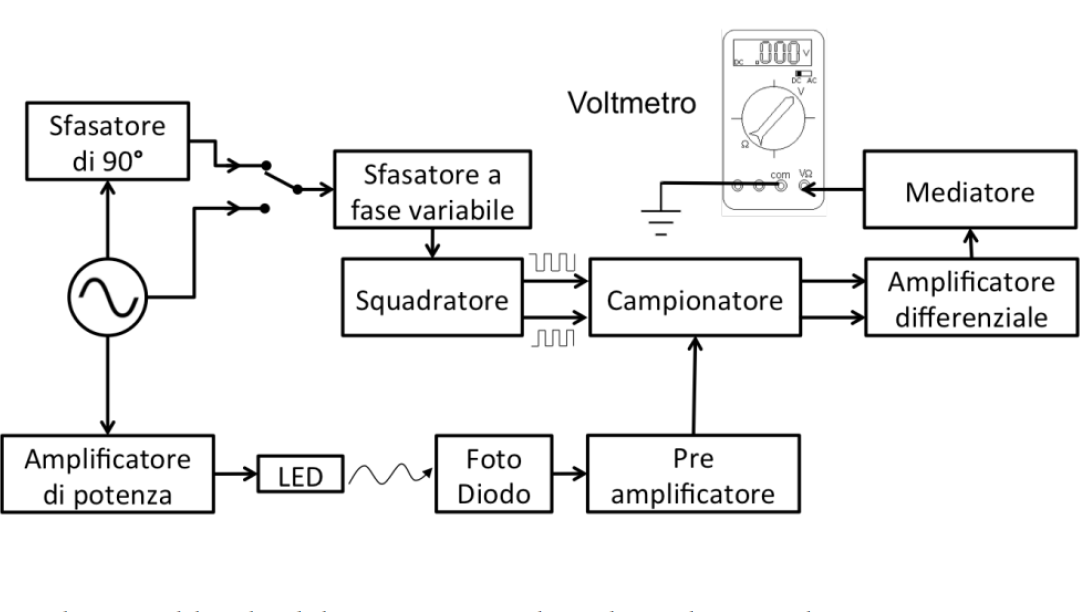
\includegraphics[scale=0.3]{./c1.png}
		\caption{scema del apparato strumentale usato.}
		\label{f:completo}
	\end{figure}